\documentclass{article}

\usepackage[margin=4cm, includefoot]{geometry}
\usepackage{graphicx}
\usepackage{float}
\usepackage{hyperref}

% Paragraph formatting
\usepackage{indentfirst}
\setlength{\parindent}{0em}
\setlength{\parskip}{1em}

% Header and footer
\usepackage{fancyhdr}
\pagestyle{fancy}
\setcounter{secnumdepth}{4}

\rhead{}
\lhead{}
\fancyfoot{}
\fancyfoot[R]{\thepage}
\renewcommand{\headrulewidth}{0pt}
\renewcommand{\footrulewidth}{0pt}
%

\begin{document}

\begin{titlepage}
	\begin{center}
		\line(1,0){400}\\
		[6mm]
		\huge{\bfseries Architectural and Functional Requirements}\\
		\line(1,0){400}\\
			[5mm]
			
\includegraphics[width=150px]{images/AWorldOfPlants.png}
			\\
		[5mm]
		\large\textbf{Project:}\\A World of Things\\
		[3mm]
		\large\textbf{Client:}\\Julian Hambleton-Jones\\
		[3mm]
		\large \textbf{Team:}\\Funge\\
		\line(1,0){400}\\
		[5mm]
		\large \textbf{Team Members:}\\
		[3mm]
		\large 14214742 - Matthew Botha\\
		\large 14446619 - Gian Paolo Buffo\\
		\large 14027021 - Matthias Harvey\\
        \large 14035538 - Dillon Heins\\[3mm]
	\end{center}
\end{titlepage}

\cleardoublepage
\thispagestyle{empty}
\tableofcontents
\cleardoublepage
\setcounter{page}{1}

\section{Introduction}
	The Internet of Things (IoT) is a development of the Internet which involves the networking of every day physical devices allowing them to send and receive data. These devices are embedded with electronics, sensors, software as well as some form of Internet or network connectivity.


	IoT is a relatively new development and has a large possibility of becoming a ubiquitous technology as well as allowing us to view the world from a different perspective. The potential it contains for innovation is endless.


	We as a group were given the opportunity to use the Amazon Web Services (AWS) IoT platform to create an IoT project of our own desires. This document details our 'A World of Things' project.

\section{Vision}
	The aim of this project is to build an innovative Internet of Things solution through the use of the Amazon Web Services Internet of Things hardware platform as well as the Amazon Web Services Cloud.
	
	No problem was formally defined and hence it was up to us to determine what solution we would be creating. We opted to create a solution which focuses on the education of students with regard to agriculture and plant sciences. We plan to motivate students to become interested in agriculture by creating an "Internet of Plants".
	
	This involves the networking and monitoring of living plants in order to analyse aspects of their environment - such as water intake, lighting, humidity, moisture, and temperature. It also involves the controlling of the environment of the plants through the adjustment of the amount of water they receive, the wavelengths of their lights and air flow through the use of fans.
	
	Users should be able to view data gathered about their plants through the use of graphs so that they can make informed decisions about what adjustments to the environment they should make.
	
	The main purpose of the platform is to encourage younger generations to become interested in agriculture and, in doing so, help stimulate South Africa's agricultural industry. We plan to implement gamification on our platform as a way to encourage users to participate.
	
	Given enough time, AI learning could be employed to optimise the conditions under which plants grow. By combining automation and AI learning, we could create an interesting challenge for the users: Grow a plant better than our control plant grown with the help of AI.

\section{Background}
	This project is part of a Software Engineering module (COS 301) for the University of Pretoria. Our client is Julian Hambleton-Jones (AWS) and our project was to create anything we wanted using the AWS IoT platform. What we decided upon was the creation of a network of living plants which are to be analysed and looked after through the use of IoT devices and our software system.
	
\subsection{Future Business/Research Opportunities}
	Through the use of sensors to continuously monitor the environment of plants a large amount of important information can be gathered. This information can create opportunities for the learning of how particular actions affect the environment of plants.
	
	This data can also be used as training data for AI so that the controlling of the environment can be fully automated such that the AI attempts to tend to and grow a plant as best as possible.
	
	These activities could help agricultural industries to improve crop yields for an increasingly growing human population.

\subsection{The Client's Problem}
	Our client did not have a particular problem which we were required to solve however we did have one restriction: we had to make use of the AWS IoT hardware platform.
	
	Through the use of this platform we were asked to create an innovative solution to a problem. The problem we decided to tackle was the growing lack of interest of young South Africans in agriculture.
	
\section{Important Terminology}
\begin{itemize}
	\item \textbf{A World of Plants} Name of the entire system.
	\item \textbf{AWS} Amazon Web Services. A secure cloud services platform offering compute power, database storage, content delivery and other functionality.
	\item \textbf{Plant Box} The enclosure which contains the plants, with all the monitoring and automation equipment.
	\item \textbf{Achievements} Gamified awards given to users for completing certain tasks.
\end{itemize}

\section{Architecture Requirements}

\subsection{Access Channel Requirements}

\subsubsection{Human Access Channels}
Users will be able to register and log into a Web interface. From the Web interface, they can associate their own Plant Boxes, monitor conditions such as temperature and humidity, control the Plant Box conditions and view their Achievements. The Web interface should be accessible from any modern browser, such as Google Chrome, Mozilla Firefox, Microsoft Edge, Apple Safari and latest Internet Explorer. The Web interface will be designed under strict UX, UI and World Wide Web Consortium (W3C) standards. This includes a responsive design that will work on any screen size. Plant Boxes do not need to be connected to the Internet at all times - the Web interface will store the latest settings and sync them with the Plant Boxes when a connection can be established.

\subsubsection{System Access Channels}
AWS API Gateway will be used expose the system's API and map it to the serverless backend provided by AWS Lambda. MQTT messages will be used to communicate between the system backend and the individual Plant Boxes. MQTT is an ISO standard (ISO/IEC PRF 20922) publish-subscribe-based "lightweight" messaging protocol for use on top of the TCP/IP protocol. It is often used to facilitate IoT communications.

	\subsection{Quality Requirements}
		\subsubsection{Performance}
			In order to have our system be as user friendly as possible, it is important to have the user interface respond quickly with little delay. The website should load quickly and logging in and out should be as fast as possible. The response to the live feed of MQTT topic updates in the live view should be instantaneous in order to allow for an accurate live graphing of the data.
				
			On the server side, Lambda function executions and database read/writes should be speedy to ensure that bottlenecks do not occur. The response to any MQTT messages received should be instantaneous in order to process multiple MQTT messages properly.
			
		\subsubsection{Usability}
			Because our system might be used by persons not familiar with complex systems, the user interface should be intuitive and efficient to use. Users with basic computer literacy should be able to easily use the core functionality of the system with little to no extra training required. Beyond the user interface, the user manual should be clear and well laid out in order to assist with learning of the system. To further ease of use, input validation should be done on the client side as much as possible to ensure that validation is fast and does not require a server response.
			
			Error messages generated by the system while in use should be clear and informative, helping the user understand and fix any issues that may have occurred. The messages should not be too technical in nature and attempt to provide a solution to the error.
			
		\subsubsection{Reliability}
			The system should be constantly available to the user via the web portal. This means that the server should not be down at any point. In order to ensure this, there should not be a single point of failure in the system.
			
			The devices send MQTT messages on a Quality of Service level of zero (QoS 0). This means that if a message is sent but not received, it is not resent. This means that the server should always be connected and waiting for MQTT messages.
			
		\subsubsection{Scalability}
			It is important that our system be scalable in order to ensure that the system can handle a very high number of users as well as all their devices. By using Amazon Web Services' Elastic Cloud Computing (AWS EC2), the system will grow and shrink as required by the users, providing a smooth experience no matter how many users or devices are connecting to the system.
			
		\subsubsection{Flexibility}
			It is important that the system has support for many hardware components such as sensors. These technologies are advancing rapidly, therefore it should be easy to add new components to the system, without making any large changes. A user should be able to add/remove any number of devices from their account, as well as add/remove any number of sensors from each device without any affect on the system.
			
		\subsubsection{Security}
			While the system does not hold any sensitive data, it is still important to have a high level of security in the system. In order to keep the users' personal information private as well as restricting unauthorized access to the system, the system uses X.509 certificates to authorize users and devices that are connecting to the system.
			
		\subsubsection{Auditability/Monitorability}
			The system will have a very high level of monitoring and audit control. The state of the devices is constantly polled and a historical record is kept of every device. By using AWS CloudWatch, we can keep access and event logs for later auditing.
			
		\subsubsection{Integrability}
			The three main parts of the system (web interface, server and devices) are highly integrable between each other. The web interface communicates with the server and devices through exposed RESTful services, allowing it to be independent and interact with any other system so long as the systems use the same RESTful calls.
			
			The device communicates with the server and the web interface through the MQTT protocol and topics, which allows it to be decoupled from the server.
			
			The server consists of multiple services that cannot be decoupled from one another as they all use the same SDK and are designed to be used in unison.

\subsection{Integration Requirements}
\begin{itemize}
	\item \textbf{HTTP}
	
	This is the foundation of data communication for the World Wide Web. It will be used to serve the web pages to the users via a web browser.	
	\item \textbf{REST}
	
	The system's RESTful API will be exposed via AWS API Gateway. This will map API calls to the serverless backend, AWS Lambda.
	\item \textbf{TCP}
	
	The TCP protocol will be used to establish network communications between the users' computers and the system's backend, as well as between the system's backend and the users' Plant Boxes.
	\item \textbf{MQTT}
	
	MQTT is a lightweight messaging protocol that will be used as a way to facilitate two-way communication between the backend and the Plant Boxes, via TCP as described above.  
	
\end{itemize}

\subsection{Architecture Constraints}
	The following architecture constraints will be applicable:
		\begin{itemize}
			\item \textbf{Programming Languages:}
			\begin{itemize}
				\item The backend must be programmed using Java
				\item The Arduino devices must be programmed using Processing
				\item The frontend must be programmed using JavaScript
			\end{itemize}
			\item \textbf{Web Services:}
			\begin{itemize}
				\item AWS IoT hardware platform
				\item AWS cloud services
			\end{itemize}
		\end{itemize}

\section{Architecture Design}

\subsection{Infrastructure}
We will be using a cloud-based, serverless, event-driven micro-services architecture. By using a micro-services approach, we will be able to develop different parts of the system concurrently, due to the loose coupling between components. This also allows more efficient unit testing because different parts of the system can be mocked independently. 

\subsection{Services}

\subsubsection{Data gathering service}
Figure \ref{fig:data-gathering} shows the components of the data gathering service. The Plant Box consists of the plants, sensors and the physical IoT device. The sensors send readings to the IoT device every 10 seconds, which in turn updates its virtual representation on the AWS IoT platform.

\begin{figure}[h!]
  \includegraphics[width=\textwidth]{images/Services/data-gathering-service.png}
  \caption{Data Gathering Service}
  \label{fig:data-gathering}
\end{figure}

\subsubsection{Processing service}
After the data has been gathered, it will be processed by means of calculating necessary statistics over a set time period. For example, every 12 hours the max, min and average readings from the temperature sensor are calculated and stored using the Database service (see section \ref{sec:database-service}). This is shown at a high level in Figure \ref{fig:processing-service}

\begin{figure}[h!]
  \includegraphics[width=\textwidth]{images/Services/processing-service.png}
  \caption{Processing Service}
  \label{fig:processing-service}
\end{figure}

\subsubsection{Business service}
The Business Service, shown in Figure \ref{fig:business-service}, handles all user interaction and delegates it to other services. This includes all Web interface functionality such as graphing, gamification and plant management. AWS API Gateway is used to map the Business service to the frontend.

\begin{figure}[h!]
  \includegraphics[width=\textwidth]{images/Services/business-service.png}
  \caption{Business Service}
  \label{fig:business-service}
\end{figure}

\subsubsection{Database service} \label{sec:database-service}
The Database Service will use the DynamoDB persistence API to persist user information and Achievements as well as plant statistics. This is illustrated at a high level in Figure \ref{fig:database-service}

\begin{figure}[h!]
  \includegraphics[width=\textwidth]{images/Services/database-service.png}
  \caption{Database Service}
  \label{fig:database-service}
\end{figure}

\subsection{Tactics}

\subsubsection{Flexibility}
\begin{itemize}
	\item Hot pluggable hardware
	\item Two-way binding of realtime updates between Web interface and hardware 
	\item Contract-based-development, which allows easy pluggability of software components via interfaces
\end{itemize}

\subsubsection{Reliability}
\begin{itemize}
	\item Ability to store latest virtual hardware state even if it is disconnected
	\item Ability to synchronise latest virtual hardware state when the physical hardware reconnects
	\item Server clustering, which ensures that the backend will never fail
	\item Database redundancy over multiple data centres to prevent a single point of failure
\end{itemize}

\subsubsection{Security}
\begin{itemize}
	\item User authentication with X.509 certificates to prevent unauthorised access
	\item Limitation of user access through User Roles with different permissions associated with them
	\item User passwords are salted and hashed before being sent over the network 
\end{itemize}

\subsubsection{Auditability}
\begin{itemize}
	\item Logging of user activity and resource usage
	\item Public access to source code and version control, which also provides transparency to users and other developers
\end{itemize}

\subsubsection{Scalability}
\begin{itemize}
	\item Processing power scales dynamically based on demand
	\item Storage capacity scales dynamically as items are added and removed
	\item Database read and write speeds scale dynamically
\end{itemize}

\section{Database and Persistence}
	The database which we are using is AWS DynamoDB. It is a managed, NoSQL database service. Some of the reasons we decided to choose a managed, NoSQL database service include, but are not limited to:
	\begin{itemize}
		\item Database operations are able to be triggered and are able to trigger other cloud services based on particular events. This suits our event-driven architecture well
		\item Automatic data replication over three availability-zones in a single region which ensures fast and redundant access
		\item It obeys a pay-per-use model
		\item Through the use of other AWS services security and access control is easy to manage
		\item "Infinitely" scalable read/write I/O running on IOPS-optimised solid state drives
	\end{itemize}

\section{Process Specification}
	In this section, there is an overview of the three main processes of the system, where each process is explained in a broad manner.
	
	\subsection{Backend}
		The backend consists of three main parts, mainly the database, the events processor and the Internet of Things (IoT) manager.
		
		\subsubsection{Database}
			The database stores the user details, which IoT device is associated with which account, as well as all the details sent by the IoT device in the updates (explained below) into the corresponding sensor detail tables. When a sensor table reaches a certain capacity, the database will trigger the events processor to collect and concatenate data into a more summarized form: hourly data is transformed into daily data, daily into monthly etc.
		
		\subsubsection{Events Processor}
		
		\subsubsection{IoT Manager}
		
	\subsection{Frontend}
		
	
	\subsection{IoT Device}

\section{Functional Requirements}
	\subsection{Use Case Prioritisation}
		\subsubsection{Critical}
			\begin{itemize}
				\item User Management Subsystem:
				\begin{itemize}
					\item Register account
					\item Login
					\item Logout
				\end{itemize}
				
				\item Plant/Device Management Subsystem:
				\begin{itemize}
					\item Create plant
					\item List plants
					\item Create and associate a virtual 'Thing' with a plant
					\item View plant status
					\item Configure light settings
				\end{itemize}
				
				\item Device Communications Subsystem
				\begin{itemize}
					\item Send readings summary to Lambda
				\end{itemize}
			\end{itemize}
		
		\subsubsection{Important}
			\begin{itemize}
				\item User Management Subsystem:
				\begin{itemize}
					\item Update User Details
				\end{itemize}
				
				\item Plant/Device Management Subsystem:
				\begin{itemize}
					\item Update plant details
					\item Configure pump settings
					\item Configure fan speeds
					\item Delete plant
				\end{itemize}
			\end{itemize}
			
		\subsubsection{Nice-to-haves}
			\begin{itemize}
				\item User Management Subsystem
					\begin{itemize}
						\item View gamification information/get user details
					\end{itemize}
				\item Device Communications Subsystem
					\begin{itemize}
						\item Complex event processing on device communications
					\end{itemize}
			\end{itemize}

\subsection{Use Case/Service Contracts}

\subsubsection{User Management Subsystem}
	\paragraph{Register Account}\mbox{}\\
		\textbf{Description:} A user must register an account before being able to access the system so that they may associated devices and plants with their account.\\
		\textbf{Prioritisation:} Critical\\		
		\textbf{Pre-conditions:}
			\begin{itemize}
				\item Email must be unique, obey email standards and not be null
				\item Username must be unique and not null
				\item Password must be longer than 8 characters and must not be null
			\end{itemize}
		\textbf{Post-conditions:}
			\begin{itemize}
				\item The password must be encrypted using PBKDF2WithHmacSHA1 and salted
				\item An identity ID must be created for the user
				\item All the above information must be associated with the username provided and stored in a database
			\end{itemize}

		\begin{figure}[H]
			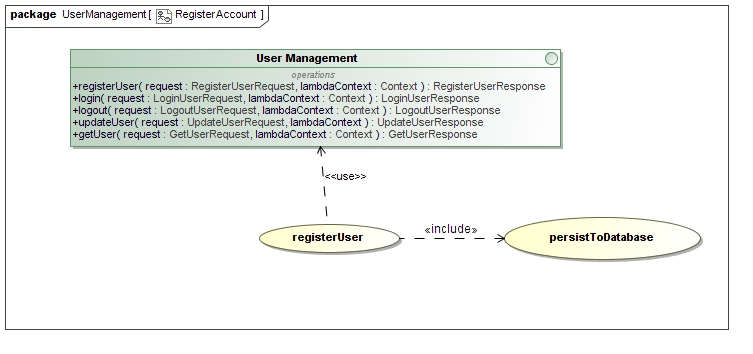
\includegraphics[width=\linewidth]{images/UseCases/RegisterAccount.jpg}
			\caption{Use case diagram for registering an account}
		\end{figure}	
		
		\begin{figure}[H]
			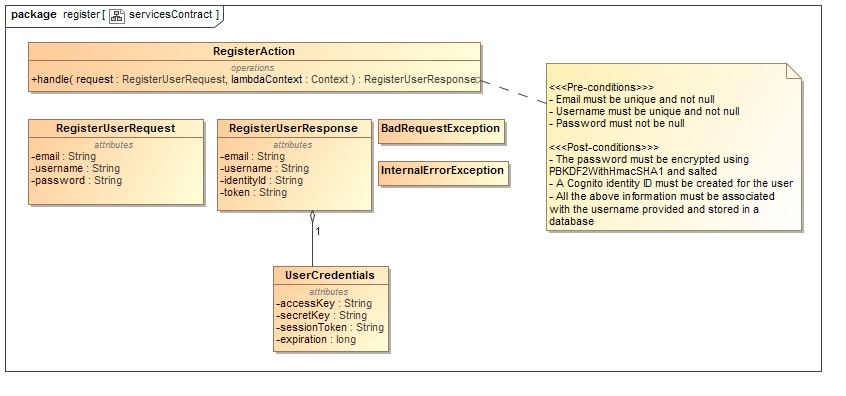
\includegraphics[width=\linewidth]{images/ServicesContracts/register.jpg}
			\caption{Services contract diagram for registering an account}
		\end{figure}
		
	\paragraph{Login}\mbox{}\\
		\textbf{Description:} A registered user must be able to login so they may securely view their account and all associated details.\\
		\textbf{Prioritisation:} Critical\\		
		\textbf{Pre-conditions:}
			\begin{itemize}
				\item Username must not be null
				\item Password must not be null
				\item User account associated with username must exist
				\item The password after being hashed and salted must match that of the provided username
			\end{itemize}
		\textbf{Post-conditions:}
			\begin{itemize}
				\item The user should be given temporary user credentials in a response object
				\item The user should be given access to their information and redirected to their dashboard
			\end{itemize}

		\begin{figure}[H]
			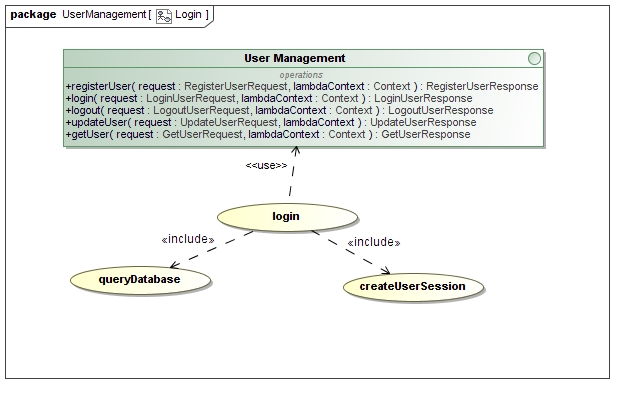
\includegraphics[width=\linewidth]{images/UseCases/Login.jpg}
			\caption{Use case diagram for login}
		\end{figure}		
		
		\begin{figure}[H]
			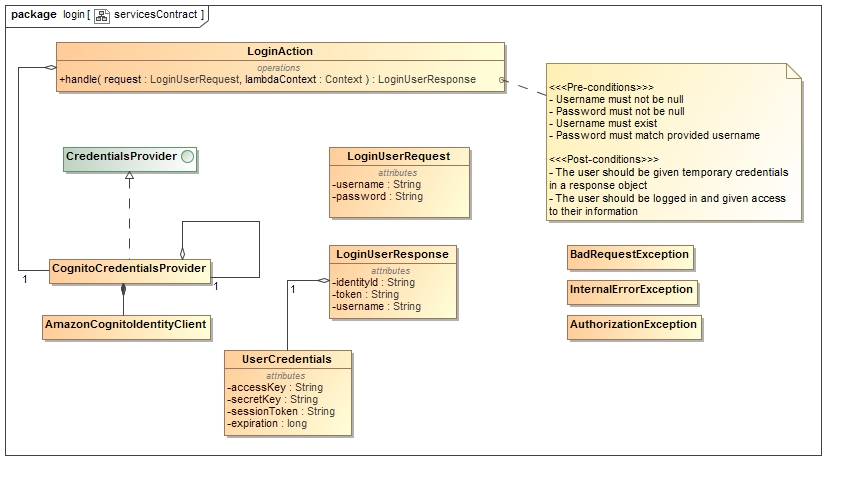
\includegraphics[width=\linewidth]{images/ServicesContracts/login.jpg}
			\caption{Services contract diagram for login}
		\end{figure}
		
	\paragraph{Logout}\mbox{}\\
		\textbf{Description:} A registered user must be able to logout securely from the system.\\
		\textbf{Prioritisation:} Critical\\		
		\textbf{Pre-conditions:}
		\begin{itemize}
			\item A user must be registered on the system
			\item The user must be logged into the system
		\end{itemize}
		\textbf{Post-conditions:}
		\begin{itemize}
			\item The user should be no longer logged into the system and as such not be able to access any functionality from the system except to register an account or log in
			\item If the user wishes to access their account and the functionality of the system, they should have to log back into the system
		\end{itemize}
		
		\begin{figure}[H]
			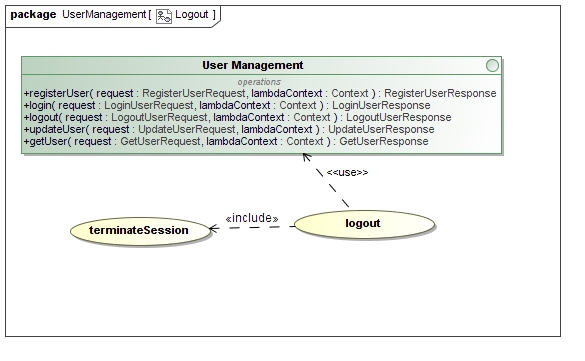
\includegraphics[width=\linewidth]{images/UseCases/Logout.jpg}
			\caption{Use case diagram for logout}
		\end{figure}		
		
		\begin{figure}[H]
			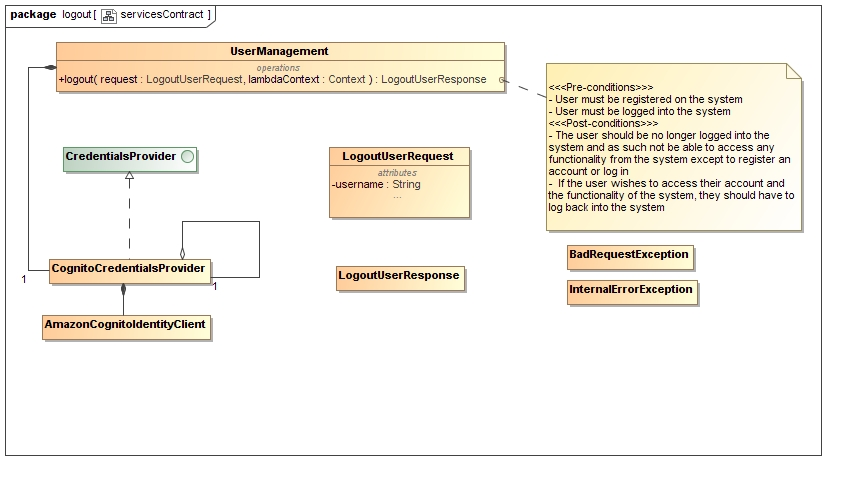
\includegraphics[width=\linewidth]{images/ServicesContracts/logout.jpg}
			\caption{Services contract diagram for logout}
		\end{figure}
		
	\paragraph{Update User Details}\mbox{}\\
		\textbf{Description:} A registered and logged in user should be able to edit details such as their email and password.\\
		\textbf{Prioritisation:} Important\\		
		\textbf{Pre-conditions:}
			\begin{itemize}
				\item User must be logged in
				\item User editing details should be the owner of those details
			\end{itemize}
		\textbf{Post-conditions:}
			\begin{itemize}
				\item The values of the edited details should be reflected in the database
			\end{itemize}

		\begin{figure}[H]
			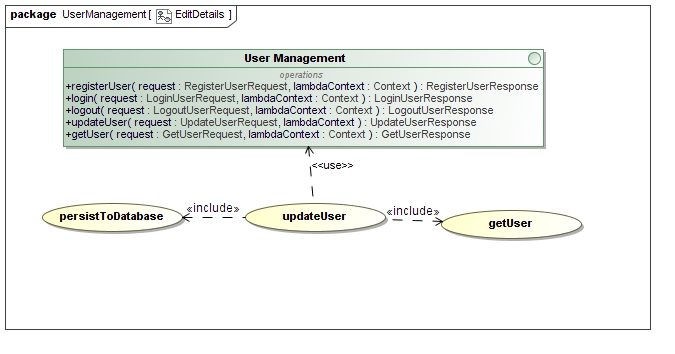
\includegraphics[width=\linewidth]{images/UseCases/EditDetails.jpg}
			\caption{Use case diagram for update user details}
		\end{figure}		
		
		\begin{figure}[H]
			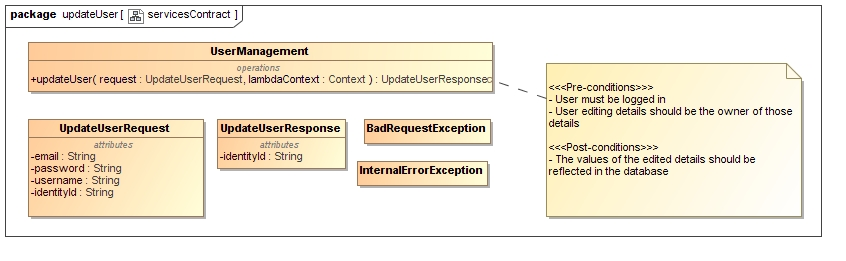
\includegraphics[width=\linewidth]{images/ServicesContracts/updateUser.jpg}
			\caption{Services contract diagram for update user details}
		\end{figure}
	
	\paragraph{View Gamification Details/Get User Details}\mbox{}\\
		\textbf{Description:} A registered and logged in user should be able to view details with regard to the progress they have made. This includes details such as their ranked level and experience points for completing tasks.\\
		\textbf{Prioritisation:} Nice-to-have\\		
		\textbf{Pre-conditions:}
			\begin{itemize}
				\item User must be logged in
			\end{itemize}
		\textbf{Post-conditions:}
			\begin{itemize}
				\item The user's personal details should be returned (username \& email)
				\item The gamification values associated with the user should be displayed to the user (level and experience)
			\end{itemize}

		\begin{figure}[H]
			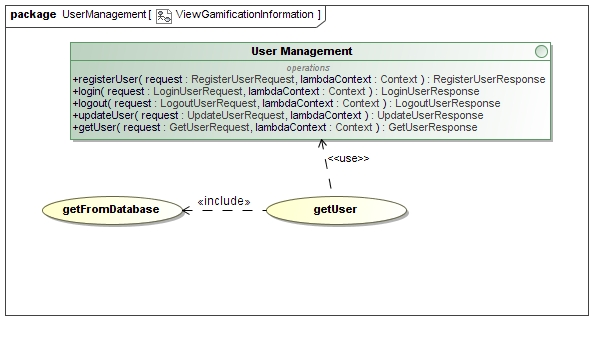
\includegraphics[width=\linewidth]{images/UseCases/ViewGamificationInformation.jpg}
			\caption{Use case diagram for view gamification details/get user details}
		\end{figure}
		
		\begin{figure}[H]
			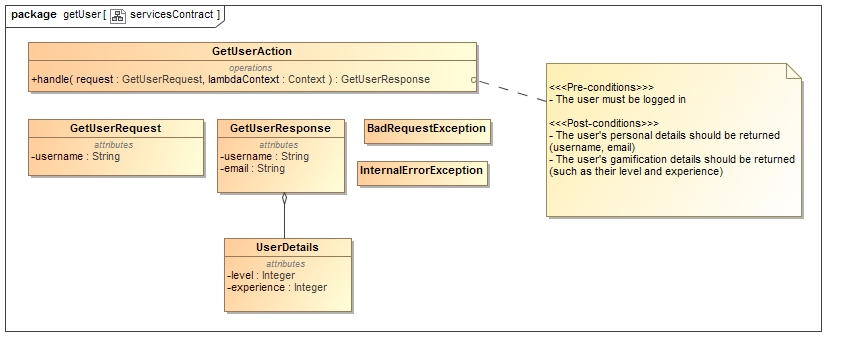
\includegraphics[width=\linewidth]{images/ServicesContracts/getUser.jpg}
			\caption{Services contract diagram for view gamification details/get user details}
		\end{figure}

\subsubsection{Plant/Device Management Subsystem}
	\paragraph{Create Plant}\mbox{}\\
		\textbf{Description:} A registered and logged in user should be able to create a virtual plant to be associated with a device monitoring a plant. This plant should have a name as well as a plant type.\\
		\textbf{Prioritisation:} Critical\\		
		\textbf{Pre-conditions:}
			\begin{itemize}
				\item The user should be logged in
				\item The plant's name should not be null
				\item The plant's type should not be null
				\item The plant's age should not be null
				\item An IoT device should be selected to be associated with the plant
			\end{itemize}
		\textbf{Post-conditions:}
			\begin{itemize}
				\item The plant should be assigned a unique identifier
				\item It should be associated with a particular user
				\item An IoT device ID should be associated with the plant
				\item The plant should be persisted in the database with all the above information
			\end{itemize}

		\begin{figure}[H]
			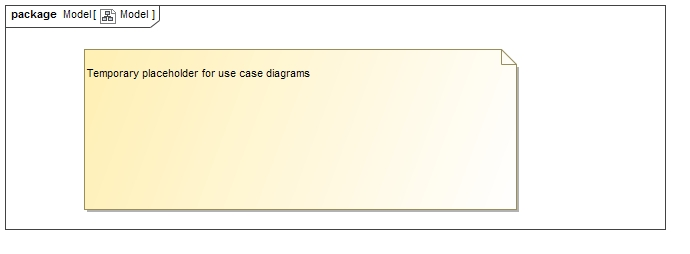
\includegraphics[width=\linewidth]{images/tempUseCase.jpg}
			\caption{Use case diagram for create plant}
		\end{figure}
		
		\begin{figure}[H]
			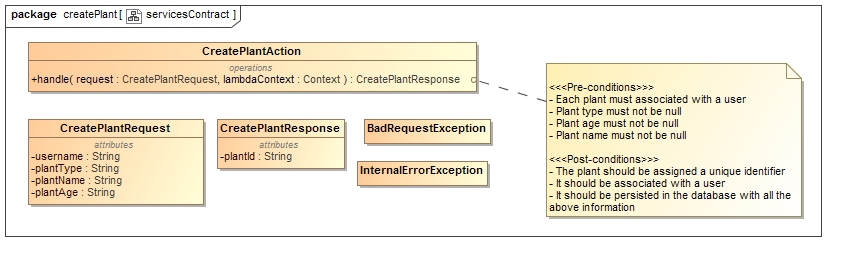
\includegraphics[width=\linewidth]{images/ServicesContracts/createPlant.jpg}
			\caption{Services contract diagram for create plant}
		\end{figure}
		
	\paragraph{List Plants}\mbox{}\\
		\textbf{Description:} A registered and logged in user should be able to retrieve a list of all the plants associated with their account.\\
		\textbf{Prioritisation:} Critical\\		
		\textbf{Pre-conditions:}
			\begin{itemize}
				\item The user should be logged in
				\item Username must not be null
			\end{itemize}
		\textbf{Post-conditions:}
			\begin{itemize}
				\item A count of the plants belonging to the supplied username should be returned
				\item A limit to the amount of plants returnable should be provided
				\item A response object containing a list of all plants associated with a user and all their individual details should be returned
			\end{itemize}

		\begin{figure}[H]
			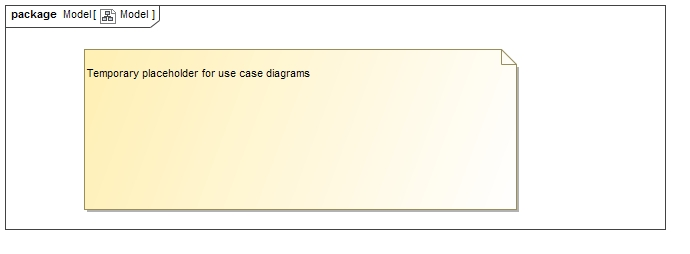
\includegraphics[width=\linewidth]{images/tempUseCase.jpg}
			\caption{Use case diagram for list plants}
		\end{figure}
		
		\begin{figure}[H]
			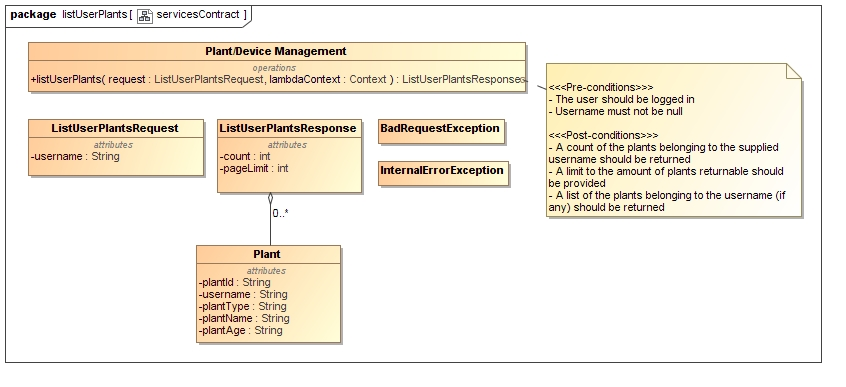
\includegraphics[width=\linewidth]{images/ServicesContracts/listUserPlants.jpg}
			\caption{Services contract diagram for list plants}
		\end{figure}
	
	\paragraph{Create and Associate a Virtual 'Thing' With a Plant}\mbox{}\\
		\textbf{Description:} A registered and logged in user should be able to create a virtual 'Thing' and associate it with a particular plant.\\
		\textbf{Prioritisation:} Critical\\		
		\textbf{Pre-conditions:}
			\begin{itemize}
				\item The user should be logged in
				\item A plant ID should be supplied
				\item The virtual 'Thing' should be associated with a particular plant
			\end{itemize}
		\textbf{Post-conditions:}
			\begin{itemize}
				\item A newly created 'Thing' should be created
				\item A relationship between the 'Thing' and a plant should be created and persisted in the database
			\end{itemize}

		\begin{figure}[H]
			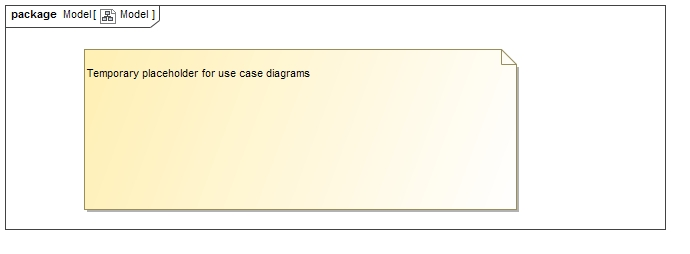
\includegraphics[width=\linewidth]{images/tempUseCase.jpg}
			\caption{Use case diagram for create and associate a virtual 'Thing' with a plant}
		\end{figure}
		
		\begin{figure}[H]
			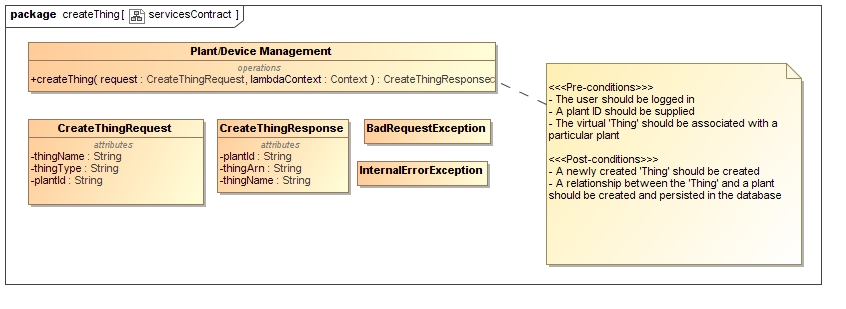
\includegraphics[width=\linewidth]{images/ServicesContracts/createThing.jpg}
			\caption{Services contract diagram for create and associate a virtual 'Thing' with a plant}
		\end{figure}
		
	\paragraph{View Plant Status}\mbox{}\\
		\textbf{Description:} A registered and logged in user should be able to view the details associated with a particular plant in terms of the readings the associated IoT device has stored in the database.\\
		\textbf{Prioritisation:} Critical\\		
		\textbf{Pre-conditions:}
			\begin{itemize}
				\item The user should be logged in
				\item A valid plantId should be supplied
			\end{itemize}
		\textbf{Post-conditions:}
			\begin{itemize}
				\item All details associated with a particular plant and gathered by the associated IoT device should be displayed. These details could include:
				\begin{itemize}
					\item Temperature
					\item Humidity
					\item Light conditions
					\item Water flow
					\item Soil moisture
				\end{itemize}
			\end{itemize}

		\begin{figure}[H]
			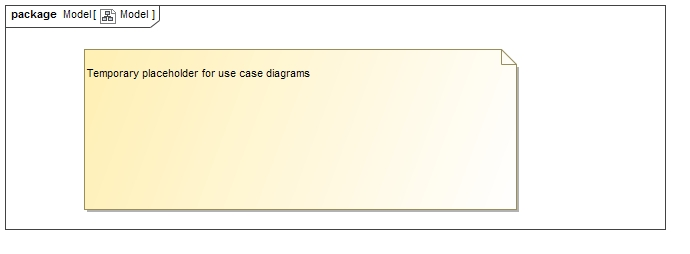
\includegraphics[width=\linewidth]{images/tempUseCase.jpg}
			\caption{Use case diagram for view plant status}
		\end{figure}
		
		\begin{figure}[H]
			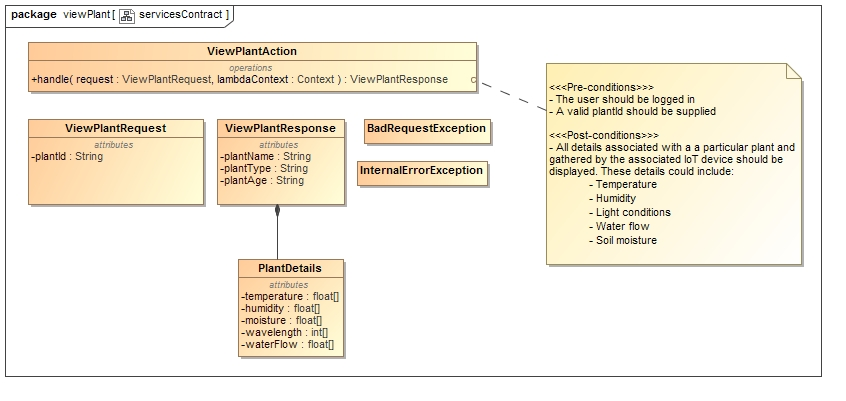
\includegraphics[width=\linewidth]{images/ServicesContracts/viewPlant.jpg}
			\caption{Services contract diagram for view plant status}
		\end{figure}
		
	\paragraph{Configure Light Settings}\mbox{}\\
		\textbf{Description:} A registered and logged in user should be able to adjust the RGB values of the LED strip associated with their IoT device via the frontend interface.\\
		\textbf{Prioritisation:} Critical\\		
		\textbf{Pre-conditions:}
			\begin{itemize}
				\item The user should be logged in
				\item A particular plant should be selected
				\item An RGB value should be specified
			\end{itemize}
		\textbf{Post-conditions:}
			\begin{itemize}
				\item The RGB value should be communicated to the device
				\item The IoT device should subsequently reflect this RGB colour in the wavelengths of the LED strip, if the RGB value was (0, 0, 0) the lights should be turned off
				\item A response object indicating whether the action was successful should be returned
			\end{itemize}

		\begin{figure}[H]
			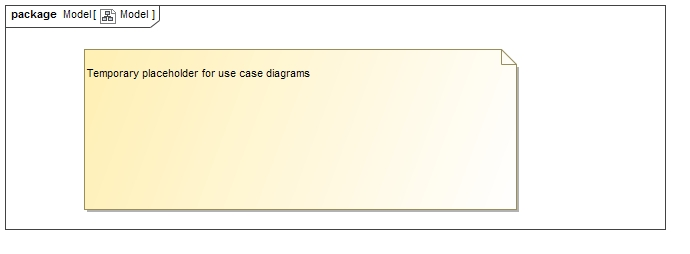
\includegraphics[width=\linewidth]{images/tempUseCase.jpg}
			\caption{Use case diagram for configure light settings}
		\end{figure}
		
		\begin{figure}[H]
			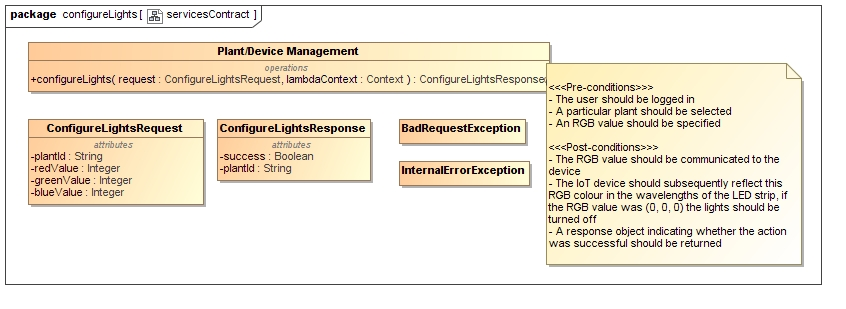
\includegraphics[width=\linewidth]{images/ServicesContracts/configureLights.jpg}
			\caption{Services contract diagram for configure light settings}
		\end{figure}
		
	\paragraph{Update Plant Details}\mbox{}\\
		\textbf{Description:} A registered and logged in user should be able to edit the name and type of a particular plant.\\
		\textbf{Prioritisation:} Important\\		
		\textbf{Pre-conditions:}
			\begin{itemize}
				\item The user should be logged in
				\item The plant ID must not be null
				\item The relevant updated information must be supplied
				\item The plant must exist
			\end{itemize}
		\textbf{Post-conditions:}
			\begin{itemize}
				\item The plant associated with the supplied plant ID must have its details updated in the database
				\item A response object indicating the operation was successful must be sent back to the client
			\end{itemize}

		\begin{figure}[H]
			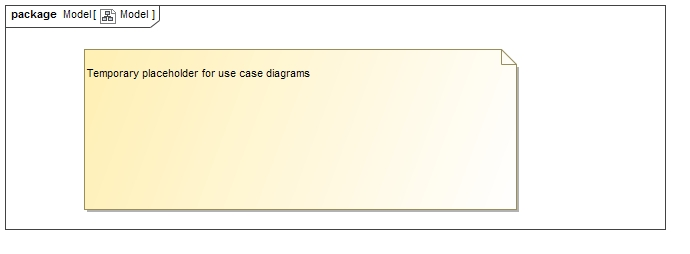
\includegraphics[width=\linewidth]{images/tempUseCase.jpg}
			\caption{Use case diagram for update plant details}
		\end{figure}
		
		\begin{figure}[H]
			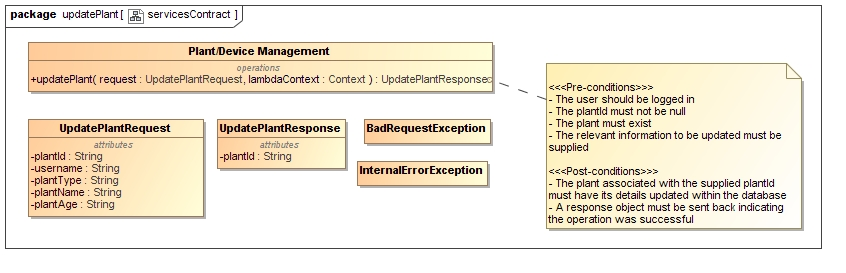
\includegraphics[width=\linewidth]{images/ServicesContracts/updatePlant.jpg}
			\caption{Services contract diagram for update plant details}
		\end{figure}		
		
	\paragraph{Configure Pump Settings}\mbox{}\\
		\textbf{Description:} A registered and logged in user should be able to configure the settings of the water pump associated with an IoT device.\\
		\textbf{Prioritisation:} Important\\		
		\textbf{Pre-conditions:}
			\begin{itemize}
				\item The user should be logged in
				\item A particular plant should be selected
				\item The configuration details should be specified
			\end{itemize}
		\textbf{Post-conditions:}
			\begin{itemize}
				\item The configuration should be communicated to and applied on the IoT device, the pump should run for the specified amount of time
				\item If the pumpTime value was 0 the pump should turn itself off
				\item A response object indicating whether the action was successful should be returned
			\end{itemize}

		\begin{figure}[H]
			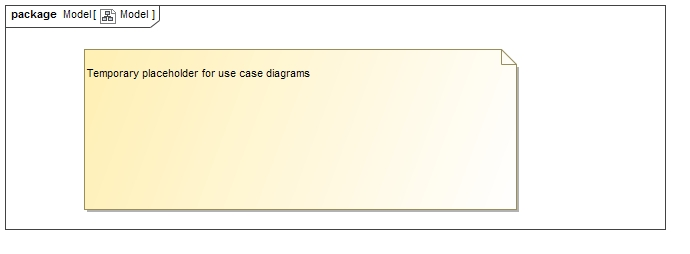
\includegraphics[width=\linewidth]{images/tempUseCase.jpg}
			\caption{Use case diagram for configure pump settings}
		\end{figure}
		
		\begin{figure}[H]
			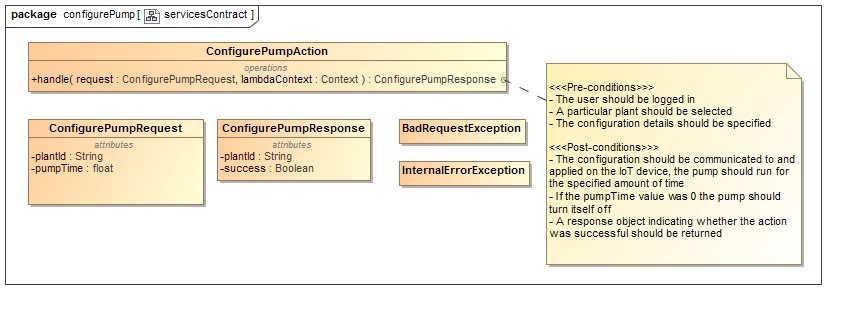
\includegraphics[width=\linewidth]{images/ServicesContracts/configurePump.jpg}
			\caption{Services contract diagram for configure pump settings}
		\end{figure}
	
	\paragraph{Configure Fan Speeds}\mbox{}\\
		\textbf{Description:} A registered and logged in user should be able to configure the settings of the fan associated with an IoT device.\\
		\textbf{Prioritisation:} Important\\		
		\textbf{Pre-conditions:}
			\begin{itemize}
				\item The user should be logged in
				\item A particular plant should be selected
				\item The configuration details should be specified
			\end{itemize}
		\textbf{Post-conditions:}
			\begin{itemize}
				\item The configuration details should be communicated to and applied on the IoT device
				\item A response object indicating whether the action was successful should be returned
			\end{itemize}

		\begin{figure}[H]
			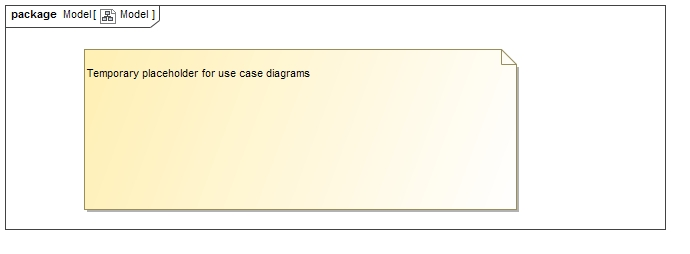
\includegraphics[width=\linewidth]{images/tempUseCase.jpg}
			\caption{Use case diagram for configure fan settings}
		\end{figure}
		
		\begin{figure}[H]
			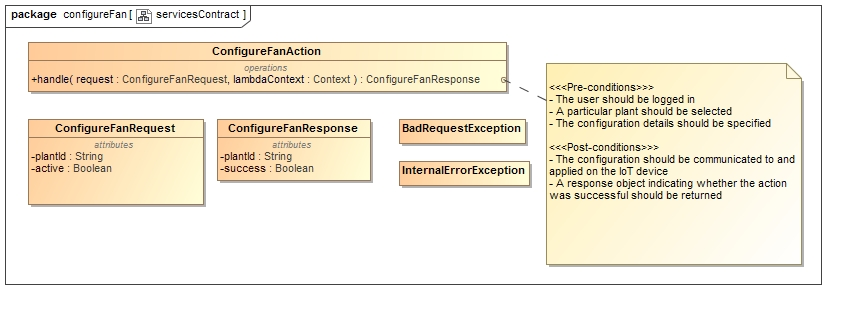
\includegraphics[width=\linewidth]{images/ServicesContracts/configureFan.jpg}
			\caption{Services contract diagram for configure fan settings}
		\end{figure}
	
	\paragraph{Delete Plant}\mbox{}\\
		\textbf{Description:} A registered and logged in user should be able to remove a plant associated with their account.\\
		\textbf{Prioritisation:} Important\\		
		\textbf{Pre-conditions:}
			\begin{itemize}
				\item The user should be logged in
				\item A particular plant should be selected
				\item The user should be the owner of the plant
			\end{itemize}
		\textbf{Post-conditions:}
			\begin{itemize}
				\item The plant's entry should be removed from the database
				\item Any information related to the plant must also be removed from the relevant tables
			\end{itemize}

		\begin{figure}[H]
			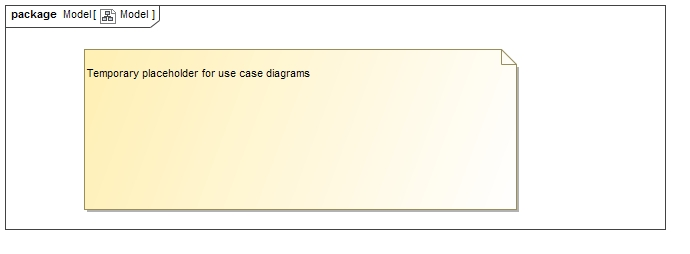
\includegraphics[width=\linewidth]{images/tempUseCase.jpg}
			\caption{Use case diagram for delete plant}
		\end{figure}
		
		\begin{figure}[H]
			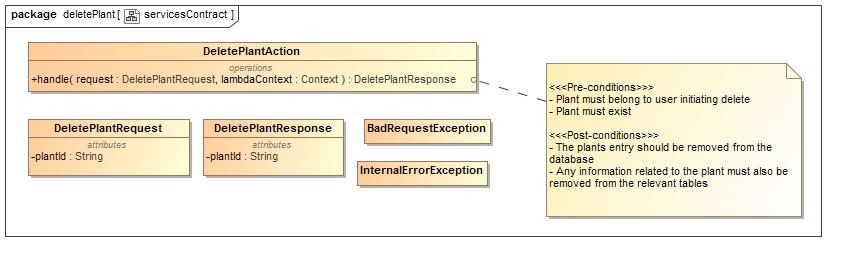
\includegraphics[width=\linewidth]{images/ServicesContracts/deletePlant.jpg}
			\caption{Services contract diagram for delete plant}
		\end{figure}
	
\subsubsection{Device Communications Subsystem}
	\paragraph{Send Readings Summary to Lambda}\mbox{}\\
		\textbf{Description:}An IoT device should send details about the information it has gathered using its sensors to the serverless provider.\\
		\textbf{Prioritisation:} Critical\\		
		\textbf{Pre-conditions:}
			\begin{itemize}
				\item A connection should be established with the IoT platform
				\item The device should publish to a particular topic
			\end{itemize}
		\textbf{Post-conditions:}
			\begin{itemize}
				\item The information gathered should be stored in the database and associated with the plant associated with the IoT device
			\end{itemize}

		\begin{figure}[H]
			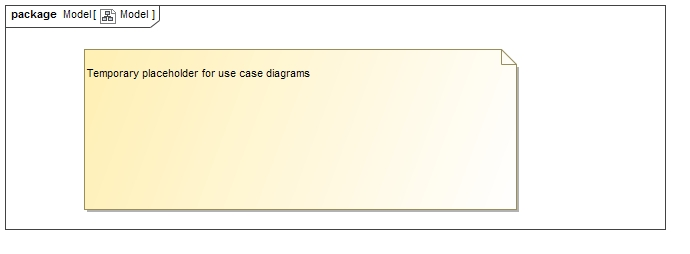
\includegraphics[width=\linewidth]{images/tempUseCase.jpg}
			\caption{Use case diagram for send readings summary to Lambda}
		\end{figure}
		
		\begin{figure}[H]
			%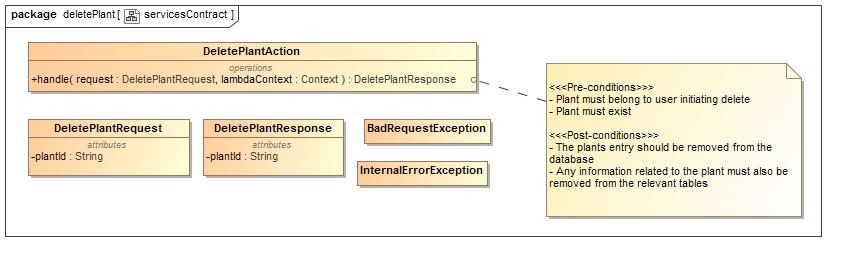
\includegraphics[width=\linewidth]{images/ServicesContracts/deletePlant.jpg}
			\caption{Services contract diagram for send readings summary to Lambda}
		\end{figure}
		
	\paragraph{Complex Event Processing on Device Communications}\mbox{}\\
		\textbf{Description:}An IoT device's readings should be intercepted and analysed to determine whether they indicate a complex event has occurred.\\
		\textbf{Prioritisation:} Critical\\		
		\textbf{Pre-conditions:}
			\begin{itemize}
				\item A connection should be established with the IoT platform
				\item The device should publish to a particular topic
				\item The information should be intercepted and analysed in real time
			\end{itemize}
		\textbf{Post-conditions:}
			\begin{itemize}
				\item According to the event the information indicates the appropriate automated action should take place in terms of controlling some aspect of the device.
			\end{itemize}

		\begin{figure}[H]
			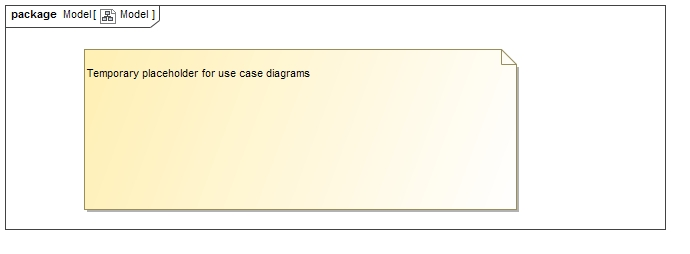
\includegraphics[width=\linewidth]{images/tempUseCase.jpg}
			\caption{Use case diagram for Complex Event Processing on Device Communications}
		\end{figure}
		
		\begin{figure}[H]
			%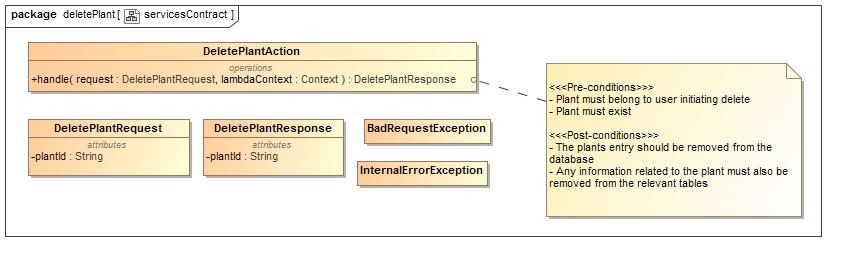
\includegraphics[width=\linewidth]{images/ServicesContracts/deletePlant.jpg}
			\caption{Services contract diagram for complex event processing on device communications}
		\end{figure}	
	
\section{Technologies}

\subsection{Todo add technologies like framework, web container etc}

\section{Initial Design}
\begin{figure}[H]
 	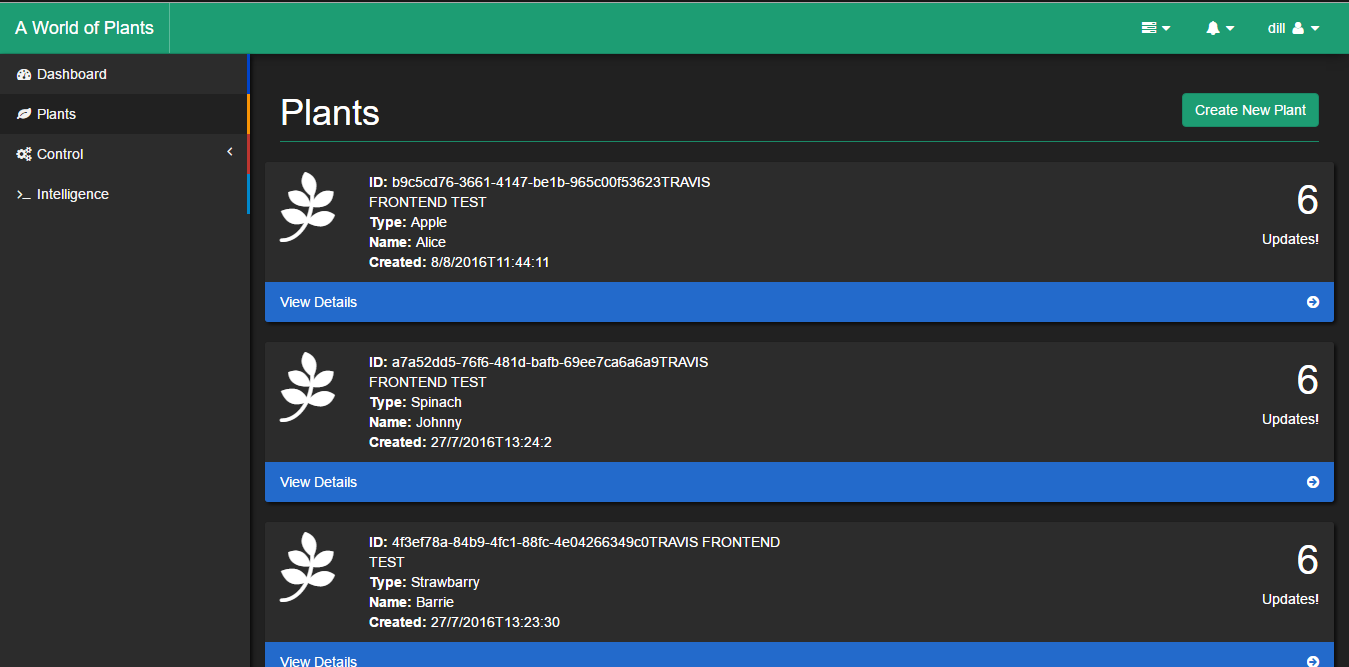
\includegraphics[width=\textwidth]{images/initial-design.PNG}
  	\caption{Initial Design of Main Interface}
\end{figure}

The initial design of the plant management section of the Web interface. Website navigation appears on the left sidebar. Notifications, Achievements and user actions appear on the top navbar. In the main section, users can add a plant and view a list of their current plants with a short overview.

\section{Open Issues}
\begin{itemize}
	\item What is the process to be followed when adding a new device?
	
	\begin{itemize}
		\item The device needs the code and certificates uploaded to it
		\item As much as possible needs to be automated for the user. Detailed steps should be given
	\end{itemize}

	\item How do you rate the conditions of the plants?
	
	Ideas:
	\begin{itemize}
		\item Using a colour palette to measure the leaf colour
		\item Getting the user to enter his analysis of the state of the plant
	\end{itemize}
	
	\item What type of gamification elements are going to be present?
\end{itemize}

\end{document}
